\section{DeepSpeech}
Mozilla DeepSpeech is an end-to-end \gls{stt} model using tensorflow. It was first developed for translating English speech to English text \cite{Hannun2014DeepSS}. \citet{Agarwal2019GermanES} have implemented a German \gls{stt} model using DeepSpeech. It is trained with machine translation techniques. They provide all of their code and pre-trained models including ready-made scripts for transfer-learning and fine-tuning (QUOTE GITHUB https://github.com/AASHISHAG/deepspeech-german). This avoids privacy issues of common web-services that require uploading potentially private data. Additionally, researchers are free to adjust and extend the model according to their requirements. DeepSpeech is a deep recurrent neural network (RNN) on character level. It can be trained using supervised learning. 

\begin{figure}[h]
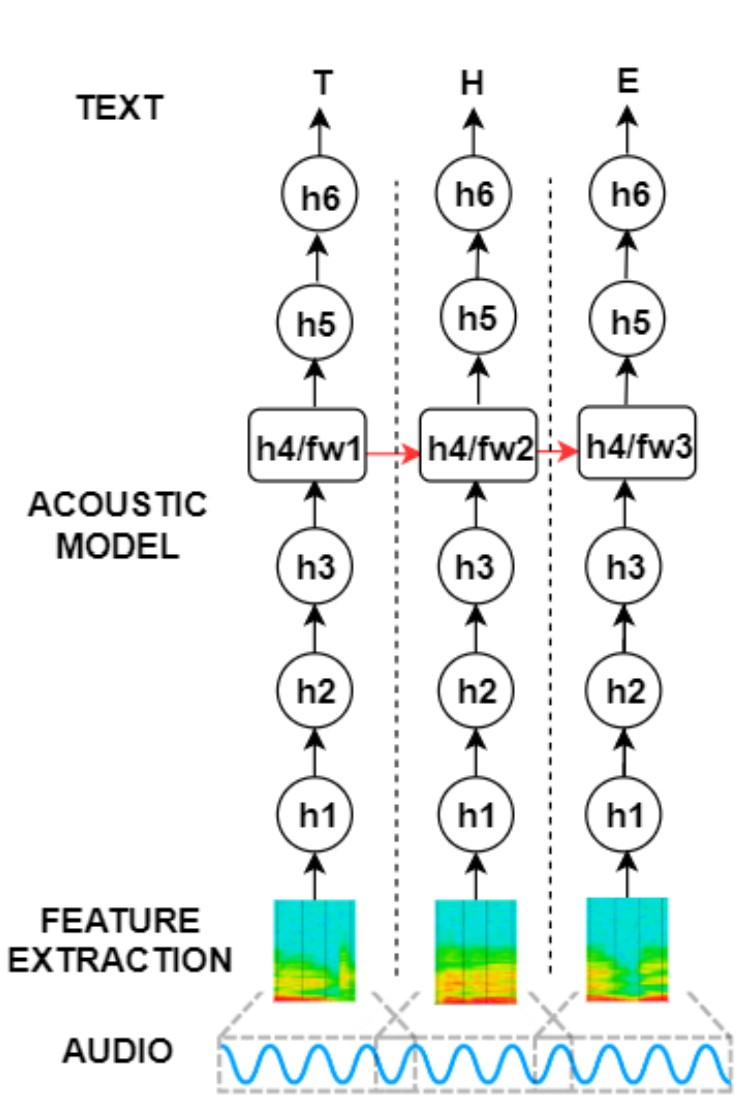
\includegraphics[scale=0.7]{deepspeech-de}
\caption{DeepSpeech architecture according to \citet{Agarwal2019GermanES}}
\label{architecture}
\end{figure}

The DeepSpeech architecture, as shown in \ref{architecture}, consists of 6 layers. A more in depth description can be found in \citet{Agarwal2019GermanES}. As becomes clear, the model has no additional phoneme-to-grapheme model but directly outputs the transcribed characters, respectively their probabilities. The Connectionist Temporal Classification (CTC) loss is used to maximize the probability of the output characters. This loss is specifically designed for tasks where the prediction categories have unclear boundaries. In this case characters which can refer to phonemes that span over times frames of various length.  